\textbf{\textit{Soal.}} Let $ABCD$ be a square and $K$ be a circle with diameter $AB$. For an arbitrary point $P$ on side $CD$, segments $AP$ and $BP$ meet $K$ again at points $M$ and $N$, respectively, and lines $DM$ and $CN$ meet at point $Q$. Prove that $Q$ lies on the circle $K$ and that $AQ : QB = DP : PC$.
\begin{proof}[\textbf{Solusi 1. }] (Friday, 11 September 2026) 
Notasikan $\measuredangle XYZ$ sebagai sudut berarah (\textit{directed angle}) yang dibentuk oleh garis $XY$ dan $YZ$.
Misalkan $O$ sebagai pusat persegi $ABCD$, $I$ dan $J$ berturut turut adalah perpotongan $AN$ dengan $BC$ dan $AD$ dengan $BM$.
\begin{center}
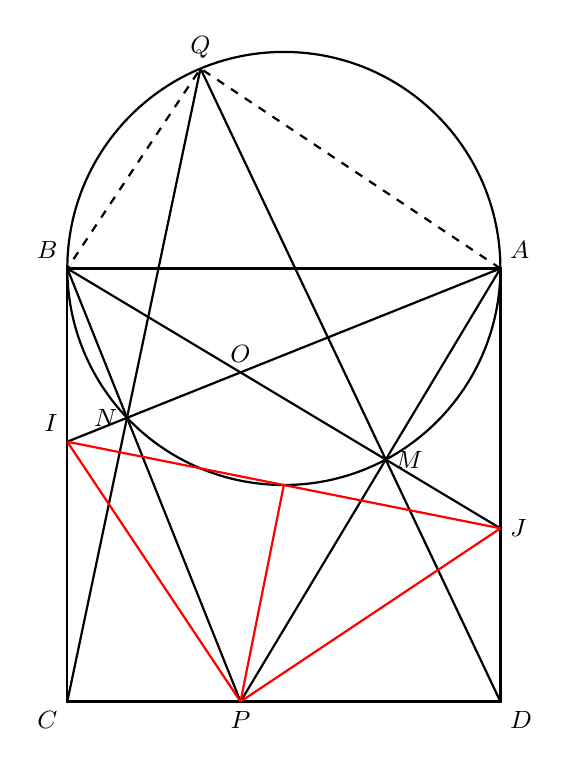
\begin{tikzpicture}[font=\small, scale=1.1]
    % Square ABCD: rotated so AB is top
    \coordinate[label=above right:$A$] (A) at (5,5);
    \coordinate[label=above left:$B$] (B) at (0,5);
    \coordinate[label=below left:$C$] (C) at (0,0);
    \coordinate[label=below right:$D$] (D) at (5,0);

    % Circle K with diameter AB
    \coordinate (CenterK) at (2.5,5);
    \draw[thick] (CenterK) circle (2.5);

    % Point P on CD, P = (2, 0)
    \coordinate[label=below:$P$] (P) at (2,0);

    % M = second intersection of AP with K
    \coordinate[label=right:$M$] (M) at (3.676, 2.794);

    % N = second intersection of BP with K
    \coordinate[label=left:$N$] (N) at (0.690, 3.276);

    % Q = DM \cap CN
    \coordinate[label=above:$Q$] (Q) at (1.538, 7.308);

    % I = AN \cap BC
    \coordinate[label=above left:$I$] (I) at (0,3);

    % J = AD \cap BM
    \coordinate[label=right:$J$] (J) at (5,2);

    % O = center of square ABCD
    \coordinate[] (O) at (2.5,2.5);

    % R = AN \cap BM
    \coordinate[label=above:$O$] (R) at (2,3.8);

    % Draw the square
    \draw[thick] (A)--(B)--(C)--(D)--cycle;

    % Draw lines AP and BP
    \draw[thick] (A)--(P);
    \draw[thick] (B)--(P);

    % Draw lines DM and CN (extended to Q)
    \draw[thick] (D)--(Q);
    \draw[thick] (C)--(Q);
    
    % Draw lines AI (which is AN extended) and BJ (which is BM extended)
    \draw[thick] (A)--(I);
    \draw[thick] (B)--(J);

    % Draw segment IJ in red
    \draw[thick, red] (I)--(J);

    % Draw segments IP, PJ, OP in red
    \draw[thick, red] (I)--(P);
    \draw[thick, red] (P)--(J);
    \draw[thick, red] (O)--(P);

    % Draw AQ and BQ to show angle AQB
    \draw[thick, dashed] (A)--(Q)--(B);

    % Mark right angles at M and N (angle in semicircle)
    % \siku{A}{M}{B}
    % \siku{A}{N}{B}
    % \siku{A}{Q}{B}

    % Draw all points
    % \foreach \s in {A,B,C,D,P,M,N,Q,I,J,O,K,L,R}
    %     \filldraw (\s) circle (1.5pt);
\end{tikzpicture}
\end{center}
Karena $AB$ diameter lingkaran $K$ maka $\measuredangle AMB = \measuredangle ANB = 90^\circ$. Maka,
\begin{align*}
    \measuredangle INP &= \measuredangle ICP = 90^\circ \iff \text{ $MJDP$ siklis dengan $PJ$ diameternya}\\
    \measuredangle JMP &= \measuredangle JDP = 90^\circ \iff \text{ $NICP$ siklis dengan $PI$ diameternya.}
\end{align*}
Sekarang, karena $AI \perp BP$ maka $\angle BAI = \angle CBP$. Karena $\angle ABI = \angle BCP = 90^\circ$, maka $\triangle ABI \cong \triangle BCP$. Dengan cara yang sama, $\triangle ABJ \cong \triangle DAP$.
Dari sini didapat $BI = CP = DJ$ dan $AJ = DP = CL$ yang mengakibatkan $\triangle PJD \cong \triangle IPC$.

Mudah didapat bahwa 
$$\dangle JPI = \dangle IPC + \dangle DPJ = 90^\circ.$$

Terakhir karena $AD \parallel BC$ maka $$\dangle CQD = \dangle JDM + \dangle NCI = \dangle JPM + \dangle NPI$$
Oleh karena itu, dapat kita lakukan sentuhan pamungkas kita:
\begin{align*}
    \dangle BQA &= \dangle BQN + \dangle MQA+ \dangle CQD\\
    &= \dangle BAN + \dangle MBA + \dangle CQD\\
    &= 90^\circ - \dangle PBA + 90^\circ - \dangle BAP + \dangle JPM + \dangle NPI\\
    &= \dangle APB + \dangle JPM + \dangle NPI\\
    &= \dangle JPI\\
    \dangle BQA &= 90^\circ.
\end{align*}
yang menunjukkan bahwa $Q$ terletak pada lingkaran $K$. Bagian pertama terbukti.

Sekarang jelas karena $\dangle AOB = 90^\circ$ maka $O$ dilewati oleh lingkaran $K$. Bagian pertama terbukti.

Selanjutnya, ingat bahwa $\angle QBA = \angle QMA = \angle DMP = \angle DJP$ yang mengakibatkan
\begin{align*}
    \dfrac{AQ}{QB} = \tan QBA = \tan DJP = \dfrac{DP}{DJ} = \dfrac{DP}{PC}
\end{align*}
sehingga terbukti juga bagian kedua. Kita selesai.
\end{proof}

\begin{proof}[\textbf{Solusi 2. }] (Friday, 11 September 2026) 
\input{TikzLatex/42 (2) Serbia TST 2004, Problem 1.tex}
Karena $K$ adalah lingkaran dengan diameter $AB$, maka $\angle AMB = \angle ANB = 90^\circ$. Untuk membuktikan $Q$ terletak pada $K$, cukup ditunjukkan $\angle AQB = 90^\circ$, atau $Q$ memenuhi persamaan lingkaran $K$.

Tanpa mengurangi keumuman, misalkan persegi \textbf{satuan} $ABCD$
\[A=(0,1),\quad B=(0,0), \quad C=(1,0), \quad D=(1,1).\]

Lingkaran $K$ berpusat di $L=\left(0,\tfrac{1}{2}\right)$ dengan jari-jari $\tfrac{1}{2}$, sehingga
\[x^2+\left(y-\tfrac{1}{2}\right)^2=\tfrac{1}{4}.\]

Misalkan $P=(1,t)$ untuk suatu $0\le t\le 1$.

Garis $AP$ dapat diparametrisasi menjadi $(s, 1-(1-t)s)$ untuk $s\ge 0$. Substitusi ke persamaan lingkaran $K$:
\begin{align*}
    s^2 + \left(\tfrac{1}{2}-(1-t)s\right)^2 &= \tfrac{1}{4}\\
    s\left((1+(1-t)^2)s - (1-t)\right) &= 0.
\end{align*}
Misalkan $u = 1-t$. Selain $s=0$ (titik $A$), didapat $s = \frac{u}{1+u^2}$, sehingga
\[M = \left(\frac{u}{1+u^2},\; \frac{1}{1+u^2}\right).\]

Lalu garis $BP$ dapat diparametrisasi sebagai $(s, ts)$ untuk $s\ge 0$. Substitusi ke persamaan lingkaran:
\begin{align*}
    s^2 + \left(ts-\tfrac{1}{2}\right)^2 &= \tfrac{1}{4}\\
    s\left((1+t^2)s - t\right) &= 0.
\end{align*}
Selain $s=0$ (yaitu titik $B$), didapat $s = \frac{t}{1+t^2}$, sehingga
\[N = \left(\frac{t}{1+t^2},\; \frac{t^2}{1+t^2}\right).\]

Sekarang, garis $DM$ dari $D=(1,1)$ dengan arah $(u^2-u+1,\; u^2)$ memiliki persamaan
\[u^2(x-1) = (u^2-u+1)(y-1).\]

Garis $CN$ dari $C=(1,0)$ dengan arah $(-(1-t+t^2),\; t^2)$ memiliki persamaan
\[t^2(x-1) = -(t^2-t+1)\,y.\]

Dari garis $CN$: $x = 1 - \frac{(t^2-t+1)}{t^2}\,y$. Substitusi ke garis $DM$ dan menggunakan $u^2-u+1 = t^2-t+1$:
\[\frac{-(1-t)^2}{t^2}\,y = y-1 \implies y = \frac{t^2}{t^2+(1-t)^2} = \frac{t^2}{2t^2-2t+1}.\]

Sehingga
\[x_Q = \frac{t(t-1)}{2t^2-2t+1}, \qquad y_Q = \frac{t^2}{2t^2-2t+1}.\]

Sekarang mari mengecek apakah $Q$ terletak pada lingkaran $K$:
\begin{align*}
    x_Q^2 + \left(y_Q - \tfrac{1}{2}\right)^2 
    &= \frac{t^2(t-1)^2}{(2t^2-2t+1)^2} + \left(\frac{2t^2 - (2t^2-2t+1)}{2(2t^2-2t+1)}\right)^2\\
    &= \frac{t^2(t-1)^2}{(2t^2-2t+1)^2} + \frac{(2t-1)^2}{4(2t^2-2t+1)^2}\\
    &= \frac{4t^2(t-1)^2 + (2t-1)^2}{4(2t^2-2t+1)^2}\\
    &= \frac{4t^4-8t^3+8t^2-4t+1}{4(2t^2-2t+1)^2}\\
    &= \frac{(2t^2-2t+1)^2}{4(2t^2-2t+1)^2} = \frac{1}{4}. \qquad \blacksquare
\end{align*}
Ternyata benar, damn.
\end{proof}

